\chapter{Setup}\label{chp:setup}
\vspace{-1em}
\begin{table}[ht]
\begin{minipage}{0.5\textwidth}
\begin{singlespace}
\begin{tabular} { cc }
      \toprule
      \textbf{Parameter} & \textbf{Values} \\ \midrule
	  Decode \& Dispatch Width & 8  \\
	  Issue Width & 8  \\
	  Execution Units & 8 \\
	  Number of Lanes & 4 \\
	  Pipeline Depth & 5 Stage \\
      L1D cache size & 32kB \\
      L1I cache size & 32kB \\
	  L1 Hit Latency & 2 Cycles \\
	  Main Memory Hit Latency & 120 Cycles\\
	  L2 cache size & 2MB \\
	  \end{tabular}
	  \end{singlespace}
\end{minipage}\hfill
\begin{minipage}{0.5\textwidth}
\begin{singlespace}
\begin{tabular} {cc }
      \toprule
      \textbf{Parameter} & \textbf{Values} \\ \midrule
	L2 Cache hit & 5-20 cycles \\
	  \# of MSHR & 8 \\
	  LSQ Organisation & Out of Order \\
	  Execution Engine & Out of Order \\
	  Branch Predictor & Tournament Style\\
	  Branch Latency & 3 Cycles \\
	  Reconfiguration Latency & 100 cycles\\
	  Processor Network & Mesh Network \\
	  Communication Latency & 1 Cycle Hop\\
	  
	  \end{tabular}
	  \end{singlespace}
\end{minipage}
\caption{Hardware characteristics of a single core of the processor.}\label{tab:processor}
\vspace{-3em}
\end{table}

\section{Dynamic Multicore Processor Simulator}\label{chp:setup:conf}

To evaluate the work a customisable cycle-level simulator for the EDGE architecture is used.
The simulator is verified against RTL implementation of an EDGE core as described in~\cite{putnam2010e2} and is within 5\% from that implementation~\cite{micolet2016dmpstream}.
This validation is done by running workloads on RTL and comparing the traces cycle-by-cycle with the simulator~\cite{micolet2017cases}.

To maintain a homogeneous view of the system, the same core configuration was used throughout the thesis.
The features of the core can be found in table~\ref{tab:processor}, and the processor is composed of 16 cores connected via a mesh network (1 cycle hop, Manhattan distance), with the L2 Cache being the shared last level cache.
The number of lanes represents how many blocks a single core can hold in its instruction window at a time, and is the same number used in the original proposal of the E2 core (4 lanes)~\cite{putnam2010e2}.

As of 2018, it is not uncommon to see embedded cores in smart-phones that have up to 12 execution units and are able to dispatch up to 6 instructions per cycle~\cite{samsung2018,apple}.
EDGE is designed to reduce the complexity and overhead of out-of-order engines by encoding dependencies at the ISA level~\cite{kim2007tflex,gray2018edge} and thus exploit high amount of instruction level parallelism with less resources.
The configuration of the core in table~\ref{tab:processor} represents an example of an EDGE core that could potentially be built today or in the near-future.
This setup was in fact described as a "small" EDGE core by Burger et al. during their keynote at ISCA 2018~\cite{iscakeynote,e2thereg,twitter}.

Chapter~\ref{chp:Background} Section~\ref{chp:Background:sec:EDGE} described how core composition is a lightweight procedure on an EDGE processor.
Therefore, for this thesis the basic reconfiguration latency is set at 100 cycles (including the pipeline flush), which is also a latency used in previously published work on core composition~\cite{pricopi2012bahurupi}.
Since the length of the reconfiguration latency can affect performance, the effect of different latencies is discussed in Chapter~\ref{chp:cases} Section~\ref{sec:dynamic}.
This is the only chapter that uses dynamic reconfiguration.
 
Previous studies on dynamic multicore processors for EDGE explored chips with up to 32 cores~\cite{kim2007tflex, gulati2008multitaskingdmc}, yet in Kim et al.'s work, they determine that 16 cores composed leads to the best average performance.
Both embedded and desktop processors are still seeing their core count rise as time goes on (Apple's A12 features 6, Huawei Mate Smart-phone has an 8 core processor, and the AMD Bulldozer features 32 cores), therefore having a 16 core EDGE processor represents a near-future design.
Also, having 16 cores available increases the number of possible configurations of the processor which in turn allows for a more impactful exploration of core composition.

\begin{figure}[t]
  \centering
    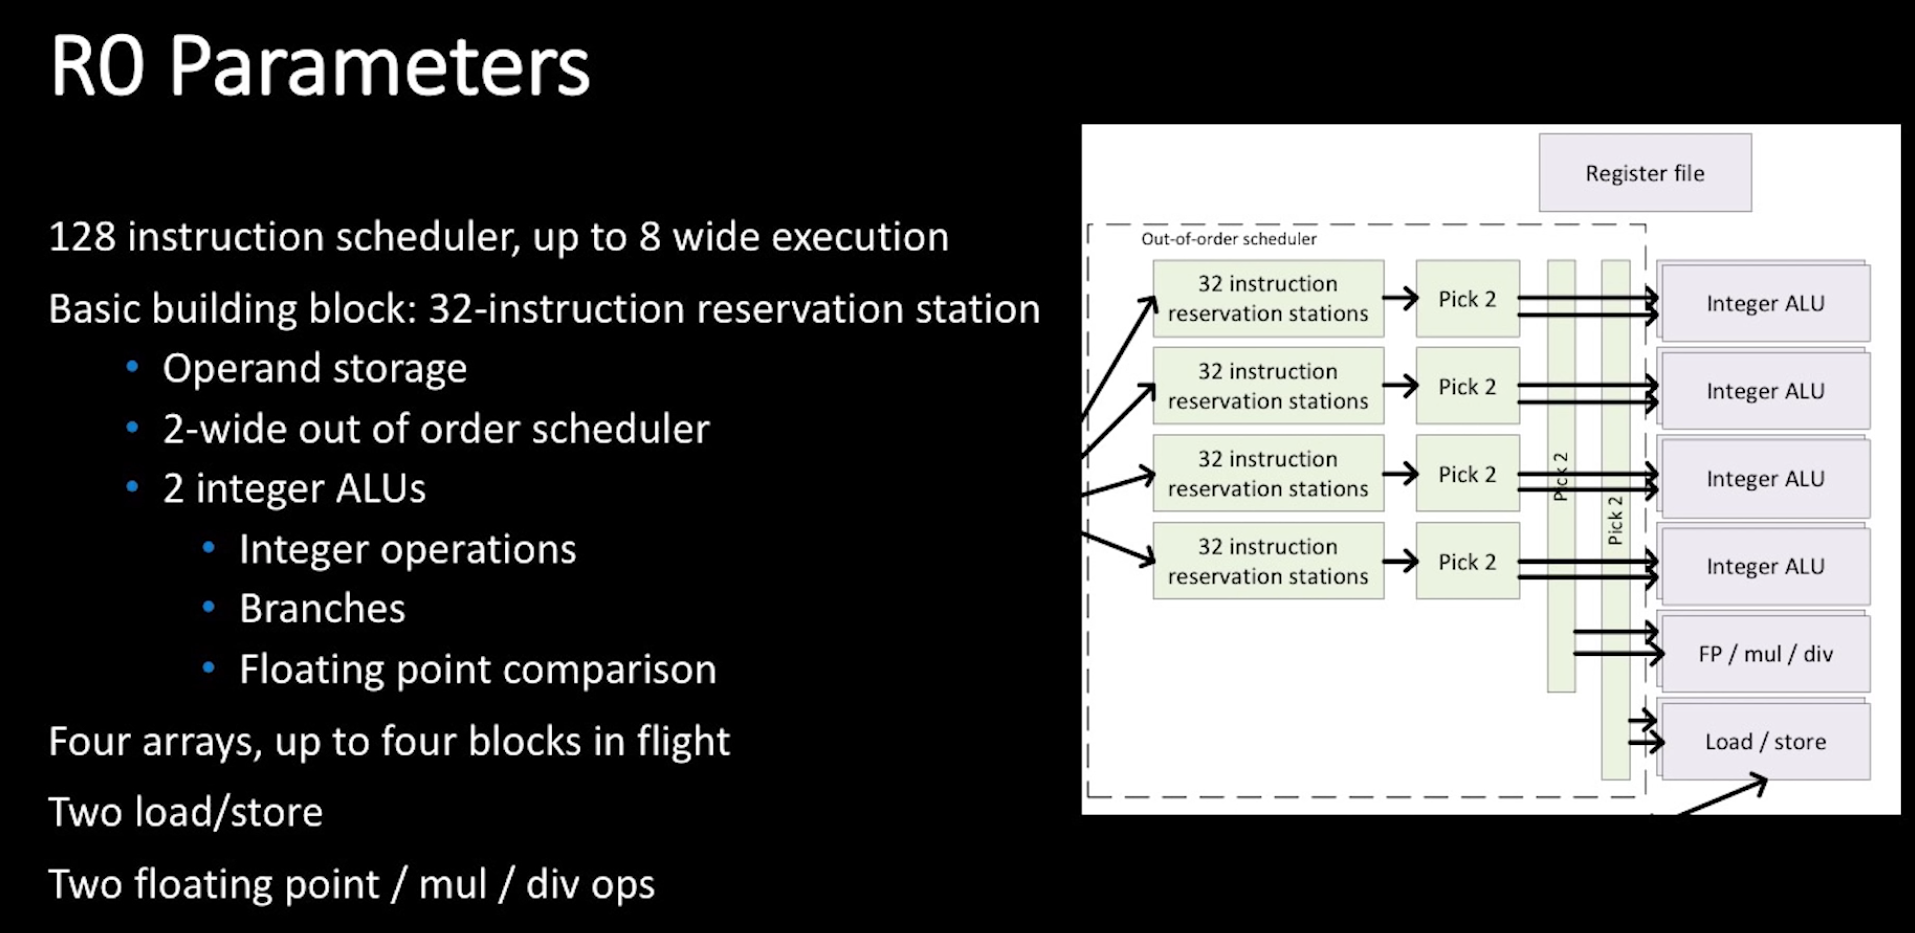
\includegraphics[width=1\textwidth]{setup/r0_parameters.png}
    \caption{Parameters of the R0 core shown by Aaron Smith during the RISE lecture}\label{fig:r0}
\end{figure}

\begin{figure}[t]
  \centering
    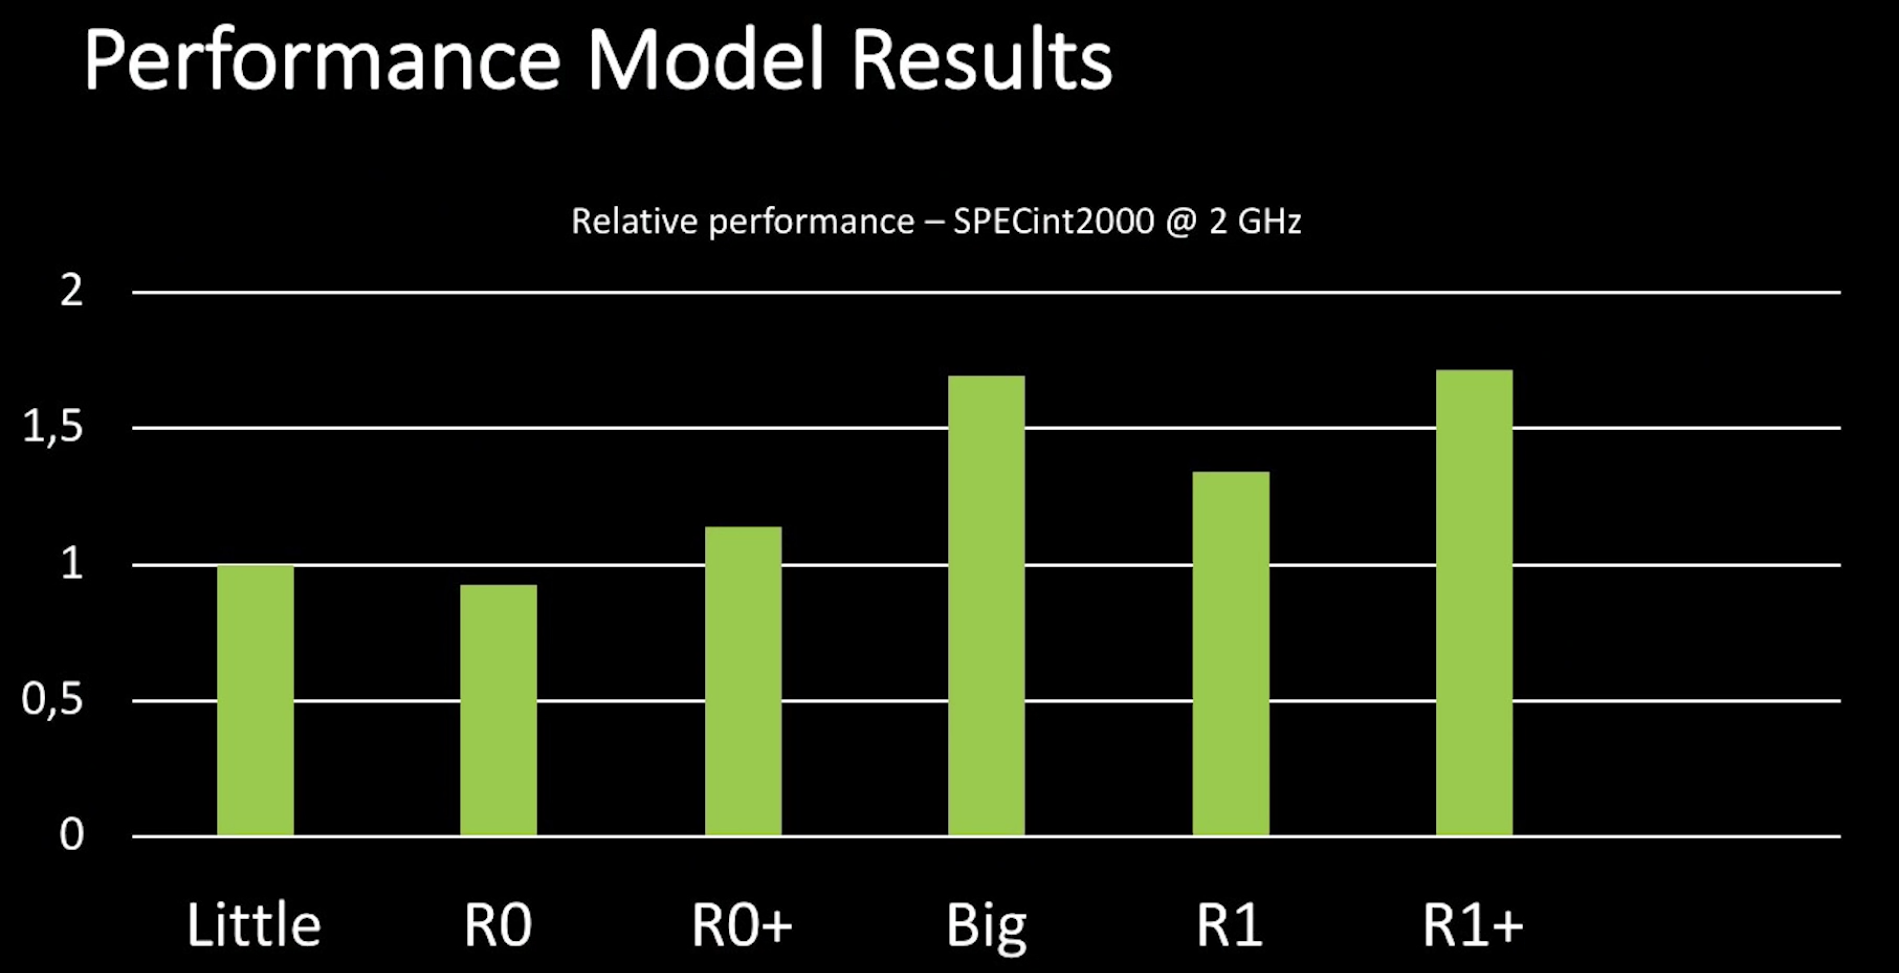
\includegraphics[width=1\textwidth]{setup/results.png}
    \caption{Performance comparison of the R0 core with a little (A53) ARM core shown by Aaron Smith during the RISE lecture. The R0+ is an refined RTL model.}\label{fig:r0perf}
\end{figure}

\subsection{Performance baseline}

In a presentation at the Research Institute of Sweden (RISE) organised by the Eurolab4HPC project~\cite{eurolab4hpc, aarontalk} , Aaron Smith presented a performance comparison of an EDGE core using the same parameters as the one used throughout this thesis with different ARM cores.
The performance comparison was conducted by Qualcomm using an RTL model of an 8 issue EDGE core (Figure~\ref{fig:r0}, and an ARM Cortex-A53 from their SnapDragon SoC~\cite{aarontalk}.
To evaluate the performance, the SPECInt2000 benchmark suite was used, and both cores were clocked at 2GHz.
As Figure~\ref{fig:r0perf} shows, a core using the parameters described in Table~\ref{tab:processor} are equivalent to that of a "little" ARM core clocked at 2GHz.

\section{Benchmarks}
This thesis explores both multi-threaded and single threaded applications to show how dynamic multicore processors (DMP) can adapt to a multitude of situations. 
This section covers the different benchmark suites used throughout the thesis.

\begin{table}[t]
\centering
% The FFT need are variable
  \smaller
 \begin{tabular} { | l | l | l | l | l | }
 \hline
  Audiobeam&   Beamformer&  Bitonic-Sort  &  BubbleSort & CFAR \\ \hline
  ChannelVocoder &  FFT& FFT3 & FFT6&  FilterBank \\ \hline
  FIR &  FMRadio &   InsertionSort &   Matmul-Block &  RadixSort\\ \hline
 \end{tabular}
  \caption{StreamIt benchmarks used in this thesis.}\label{tab:streamwl}
\end{table}

\subsection{Streaming applications}\label{chp:setup:streamit}

Chapter~\ref{chp:streamit} demonstrates how configuring a DMP to get the optimal performance out of multi-threaded applications can be learned.
To explore this concept, choosing a programming language that naturally exposes parallelism is important as it facilitates the process of generating threads for an application.
As the introduction of Chapter~\ref{chp:streamit} will explain, StreamIt is one such language.

The StreamIt repository holds a set of benchmarks that can be used to evaluate the system~\cite{streamitrepo}.
As the processor and tools used throughout this thesis are still in development, some of the applications would either not compile or execute correctly on the provided simulator; thus a subset of the applications are used.
The 15 StreamIt benchmark that worked and are explored in Chapter~\ref{chp:streamit} are shown in Table~\ref{tab:streamwl}.
These applications represent a variety of embedded applications and kernels, from digital signal processing to a matrix-multiplication kernel or band pass filters.
They can be found in a multitude of devices from digital radios to HDTVs and smart-phones (audio/video streaming applications).
The benchmarks also present a varying degree of parallelism as will be shown in Chapter~\ref{chp:streamit} Section~\ref{chp:stream:sec:setup}.
As dynamic multicore processors are intended to adapt to the program at hand, having varying amounts of parallelism in the different benchmarks is essential to demonstrate its flexibility.

\subsection{San-Diego Vision Benchmark Suite}\label{chp:setup:sdvbs}
\begin{table}[t]
  \smaller
  \centering
 \begin{tabular} { | l | l | }
 \hline
   \cellcolor[gray]{0.7}Characteristic & \cellcolor[gray]{0.7} Benchmarks\\ \hline
    Memory Intensive & Disparity, Tracking\\ \hline
	Computation Intensive & MSER, SVM, SIFT, Localization,Multi NCut\\\hline
	Memory and Computation Intensive & Stitch\\ \hline
   \end{tabular}
  \caption{Characteristics of the benchmarks~\cite{sdvbs}.}\label{tab:sd-vbschar}
\vspace{1em}
  \end{table}
  
As core composition is designed to improve the performance of single-threaded applications, it is also important to evaluate a set of serial applications.
Chapters~\ref{chp:cases} and \ref{chp:hardchanges} explore a set of Vision Benchmarks designed for hardware and compiler research~\cite{sdvbs}.
The San Diego Vision Benchmark suite (SD-VBS) is composed of nine single-threaded C benchmarks ranging from image analysis to motion tracking.
These benchmarks represent state-of-the-art applications in image and vision recognition which are prevalent in embedded systems.
The domain of image analysis and vision recognition is prevalent in multiple commercial and research fields, such as robotics, self-driving cars and even facial recognition in smart-phones.

Vision applications are usually designed as software pipelines featuring different passes which will naturally form phases throughout the execution of the program.
The programs typically have regular and simple control flow which enables the formation of large blocks of instructions.
The processor relies on the ability to form large blocks to exploit block level parallelism (BLP) which makes these applications particularly well suited.
As the results will show, the phase length has minimal impact on energy savings when the reconfiguration overhead is low.

All the benchmarks in the suite are described here:
\begin{itemize}
\item \textbf{Disparity} Computes depth information for a given pair of images.
\vspace{-1em}
\item \textbf{Localization} Estimates position of robot based on its surroundings.
\vspace{-1em}
\item \textbf{MSER} Maximally Stable Extremal Regions, a method used for blob detection in images.
\vspace{-1em}
\item \textbf{Multi NCut} Partitions images into conceptual regions.
\vspace{-1em}
\item \textbf{Sift} Scale invariant feature transform is used to extract and describe items found in an image.
\vspace{-1em}
\item \textbf{Stitch} Combines multiple photographs into a single image.
\vspace{-1em}
\item \textbf{SVM} Support Vector Machine.
\vspace{-1em}
\item \textbf{Texture Synthesis} Creates larger image out of a small sample.
\vspace{-1em}
\item \textbf{Tracking} Extracts motion information from a set of images.
\end{itemize}

and their characteristics in terms of memory/computation intensity are shown in Table~\ref{tab:sd-vbschar}.
\section{Compiler}\label{chp:setup:comp}

All the benchmarks explored in this thesis are compiled using a closed-source EDGE compiler provided by Microsoft.
The benchmarks are compiled with \textit{-O2} optimisations as this is the highest level of optimisations available with hyperblock formation turned on (it is its own separate flag).
